\documentclass{nime-alternate}
\usepackage{hyperref}
\hypersetup{colorlinks,urlcolor=blue}
\makeatletter
\DeclareUrlCommand\ULurl@@{%
  \def\UrlFont{\ttfamily\color{blue}}%
  \def\UrlLeft{\uline\bgroup}%
  \def\UrlRight{\egroup}}
\def\ULurl@#1{\hyper@linkurl{\ULurl@@{#1}}{#1}}
\DeclareRobustCommand*\ULurl{\hyper@normalise\ULurl@}
\makeatother
\usepackage{minted}
\usepackage{graphicx}
\begin{document}

\conferenceinfo{NIME'15,}{2015, Louisiana State University, USA.}

\title{Integrating internet resources and inexpensive materials to evolve a 
Raspberry Pi into a digital button sound machine. }

\numberofauthors{1}

\author{
\alignauthor
Benjamin Guitreau\\
\affaddr{Center for Communication and Technology}\\
\affaddr{Baton Rouge, Louisiana}\\
\email{bguitr1@tigers.lsu.edu}
}

\date{10 May 2014}

\maketitle
\begin{abstract}
The goal of this paper is to provide the details involved in designing and building 
a digital musical enclosure that uses a button matrix as the keys. The idea is to allow for an instrument that can be replicated by hobbyists, students, and professionals alike by using inexpensive parts, materials, and resources that are only a few keystrokes away. The project is scalable in any direction and is not limited to producing audio signals. 
\end{abstract}

\keywords{NIME, proceedings, Raspberry Pi, Sparkfun}

\section{Introduction}
The materials 
in the construction are inexpensive and accessible from online retailers such as Sparkfun\cite{SF}, while the design is straight-forward and easily reproducable or modified.. The basic programming to get the instrument working is minimal which allows for anyone to be able to write the code, while allowing for more advanced users to create complex scores.

\section{Design}

\subsection{Hardware}
The design of the box is based upon an enclosure built by Berdahl\cite{Berdahl:2014:Misc}. Using BoxMaker\cite{Bhargava:2013:Misc}, the builder is able to initiate the design process by inputting the dimensions and material thickness of the box. Using the downloaded design, the builder is able to edit the design with either Inkscape, CorelDraw, or Adobe Illustrator which allows for the creation of a project that can then be uploaded to Ponoko\cite{Ponoko}. Depending upon the material of choice, Ponoko will cut the pieces for the box and ship them to the builder.

The electronic hardware was all be purchased from the Sparkfun website for less than \$70. A Raspberry Pi\cite{RPi} is mounted inside of the box keeping the GPIO pins accessible. A button pad breakout board\cite{PCB} is mounted on the top of the box, with a silicon rubber button pad\cite{BP} placed on top of the breakout board. Soldered to the board are 16 diodes\cite{DIO} and 8 breakaway header pins\cite{BH}. Female to female jumper wires\cite{Jumper} are used to connect the header pins to the GPIO pins that will be used in the construction of the instrument. The GPIO pins and the breakout board are connected per the following figure.

\begin{figure}[h!]
\caption{GPIO-Breakout board schematic}
\label{schematic}
\centering
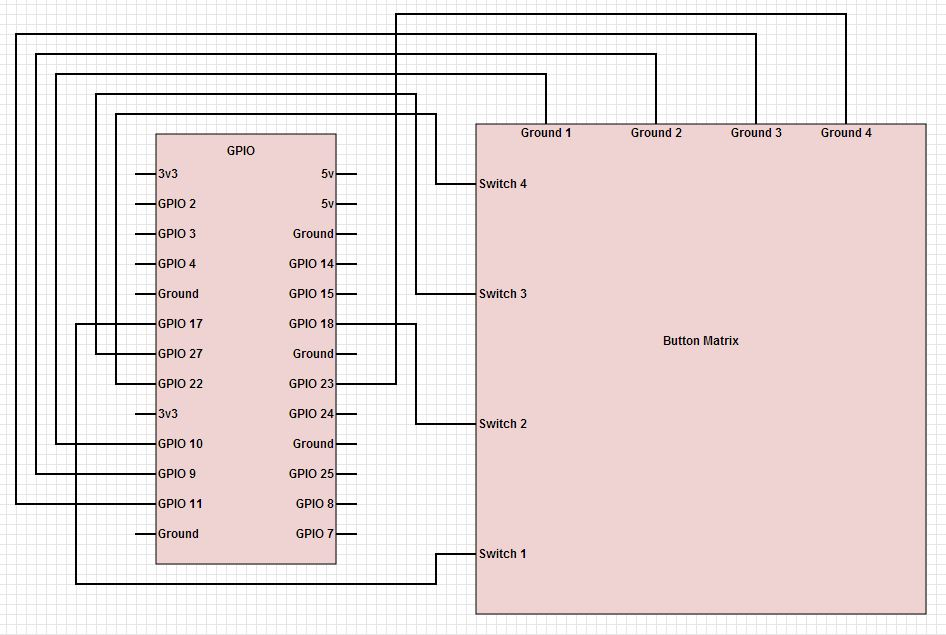
\includegraphics[height=2.5in]{ffschematic.jpg}
\end{figure}

\subsection{Software}
A python script, that is started during the bootup sequence of the Pi, is controlling the reading of the button matrix. The builder must install either python3 or python2 (python3 was used for the project and all source code available will be using python3) and RPi.GPIO\cite{RPi.GPIO} to be able to use the instrument. The Pi has internal pull-up/pull-down resistors, which are necessary to discern the button being pressed. In the snippet of code below, 3 lists are created. The first list is the matrix allocation of buttons, while the other two lists contain the GPIO pin number connected to the respective row or column. 
 
\begin{minted}[tabsize=2]{python3}
import RPi.GPIO as GPIO

class ButtonMatrix():
	BUTTON_MATRIX = [
		[1,2,3,4],
		[5,6,7,8],
		[9,10,11,12],
		[13,14,15,16]]
	ROW = [22,27,18,17]
	COLUMN = [10,9,11,23]
\end{minted}

The script initially sets GPIO column pins as output with a low value. The GPIO row pins are initially set as input with pull-up resistors. When a button is pressed, the row value is read and then the column and row settings are reversed, except instead of a low value, the row pins are set with an output at high value and the column pins are set as an input with pull-down resistors. The column value is then read and the button matrix value is calculated using the two dimensional indices of the matrix list.

Pure Data extended, or pd-extended, is running on the Pi for musical/audio generation. Python and pd are communicating using the pdsend and pdreceive. In this setting, there is no discernible latency between button presses.

\section{Conclusions}
The builder can can spend under \$100 (US) and less than a few hours of time to create a digital musical instrument. By using Ponoko, anyone can design and build the box without worrying about having access to a laser-cutter, which allows for a plethora of opportunities for younger students and hobbyists to expand upon this project.

%ACKNOWLEDGMENTS are optional
\section{Acknowledgments}
The author would like to thank Edgar Berdahl for the opportunity and support in the design and implementation.

\bibliographystyle{abbrv}
\bibliography{RPiPD_button_matrix}

\balancecolumns 

\end{document}
